\usetikzlibrary{arrows.meta,calc,shadings,fadings}

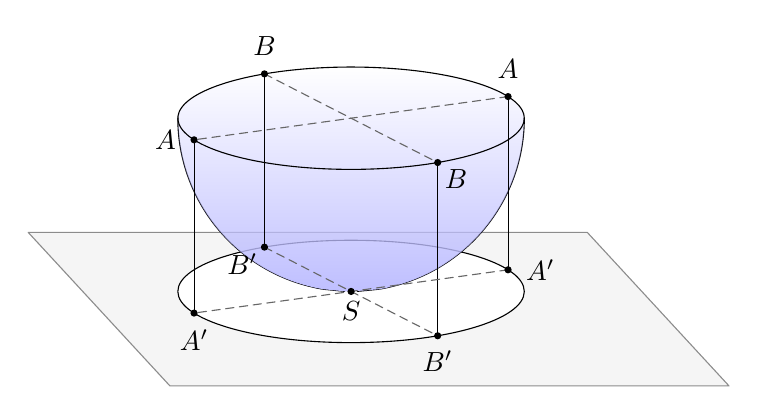
\begin{tikzpicture}[>=Stealth, line cap=round, line join=round]

% ----------------------------
% PARAMETERS
% ----------------------------
\def\a{2.2}       % ellipse x radius
\def\b{0.65}      % ellipse y radius
\def\H{2.2}       % hemisphere height
\def\Oy{-2.0}     % ground level y

\coordinate (O) at (0,\Oy);
\coordinate (Top) at (0,{\Oy+\H});   % equator center (flat top)

% ----------------------------
% ANGLES for labeled points
% ----------------------------
\def\phiA{25}     % azimuthal angle for A pair
\def\phiB{120}    % azimuthal angle for B pair

% ----------------------------
% BASE PLANE (parallelogram)
% ----------------------------
\coordinate (PL1) at (-4.1,-1.25);
\coordinate (PL2) at (3.0,-1.25);
\coordinate (PL3) at (4.8,-3.2);
\coordinate (PL4) at ($(PL1)+(PL3)-(PL2)$);

\path[fill=gray!8, draw=black!45]
  (PL1) -- (PL2) -- (PL3) -- (PL4) -- cycle;

% ----------------------------
% PROJECTION ELLIPSE (on ground plane)
% ----------------------------
\fill[white] (O) ellipse [x radius=\a, y radius=\b];
\draw (O) ellipse [x radius=\a, y radius=\b];

% ----------------------------
% SOUTHERN HEMISPHERE (dome down, equator on top)
% t: 0 = equator, 1 = south pole
% x = a * sqrt(1-t^2) * cos(phi)
% y = (Oy+H) - H*t + b * sqrt(1-t^2) * sin(phi)
% ----------------------------

% Silhouette meridians (left and right outlines)
% phi = 180 (left side)
\draw
  plot[domain=0:1, samples=80, smooth]
  ({-\a*sqrt(1 - \x*\x)},
   {\Oy + \H - \H*\x});

% phi = 0 (right side)
\draw
  plot[domain=0:1, samples=80, smooth]
  ({\a*sqrt(1 - \x*\x)},
   {\Oy + \H - \H*\x});

% Single fill with path fading: blue at bottom, transparent at top
\fill[blue!25, path fading=north]
  plot[domain=0:1, samples=80, smooth]
  ({-\a*sqrt(1 - \x*\x)}, {\Oy + \H - \H*\x})
  -- (0, \Oy)
  -- plot[domain=1:0, samples=80, smooth]
  ({\a*sqrt(1 - \x*\x)}, {\Oy + \H - \H*\x})
  -- plot[domain=0:360, samples=80, smooth]
  ({\a*cos(\x)}, {\Oy + \H + \b*sin(\x)})
  -- cycle;


% ----------------------------
% EQUATOR ELLIPSE (flat top, fully solid)
% ----------------------------
\draw
  plot[domain=0:360, samples=80, smooth]
  ({\a*cos(\x)}, {\Oy + \H + \b*sin(\x)});

% ----------------------------
% LABELED POINTS ON EQUATOR AND PROJECTIONS
% ----------------------------

% A pair (diametrically opposite on equator)
\coordinate (eqA)  at ({\a*cos(\phiA)}, {\Oy+\H+\b*sin(\phiA)});
\coordinate (eqA2) at ({-\a*cos(\phiA)}, {\Oy+\H-\b*sin(\phiA)});

% B pair (diametrically opposite on equator)
\coordinate (eqB)  at ({\a*cos(\phiB)}, {\Oy+\H+\b*sin(\phiB)});
\coordinate (eqB2) at ({-\a*cos(\phiB)}, {\Oy+\H-\b*sin(\phiB)});

% Projections on base plane
\coordinate (prA)  at ({\a*cos(\phiA)}, {\Oy+\b*sin(\phiA)});
\coordinate (prA2) at ({-\a*cos(\phiA)}, {\Oy-\b*sin(\phiA)});
\coordinate (prB)  at ({\a*cos(\phiB)}, {\Oy+\b*sin(\phiB)});
\coordinate (prB2) at ({-\a*cos(\phiB)}, {\Oy-\b*sin(\phiB)});

% Solid lines: point to its own projection
\draw (eqA)  -- (prA);
\draw (eqA2) -- (prA2);
\draw (eqB)  -- (prB);
\draw (eqB2) -- (prB2);

% Dashed lines: diametrically opposite points on equator
\draw[densely dashed, black!60] (eqA) -- (eqA2);
\draw[densely dashed, black!60] (eqB) -- (eqB2);

% Dashed lines: diametrically opposite projections
\draw[densely dashed, black!60] (prA) -- (prA2);
\draw[densely dashed, black!60] (prB) -- (prB2);

% Points on equator
\fill (eqA) circle (1.3pt);
\node[above=3pt] at (eqA) {$A$};
\fill (eqA2) circle (1.3pt);
\node[left=3pt] at (eqA2) {$A$};

\fill (eqB) circle (1.3pt);
\node[above=3pt] at (eqB) {$B$};
\fill (eqB2) circle (1.3pt);
\node[below right=-0.9pt] at (eqB2) {$B$};

% Projected points on base
\fill (prA) circle (1.3pt);
\node[right=3pt] at (prA) {$A'$};
\fill (prA2) circle (1.3pt);
\node[below=2.5pt] at (prA2) {$A'$};

\fill (prB) circle (1.3pt);
\node[below left=-1pt] at (prB) {$B'$};
\fill (prB2) circle (1.3pt);
\node[below=2pt] at (prB2) {$B'$};

% ----------------------------
% CENTER POINTS
% ----------------------------
\fill (O) circle (1.3pt);
\node[below=0pt] at (O) {$S$};

% (top center dot removed)

\end{tikzpicture}
